%%%%%%%%%%%%%%%%%%%%%%%%%%%%%%%%%%%%%%%%%%%%%%%%%%%%%%%%%%%%%%%%%%%%%%%%%%%%%%%%
% Finite State Machine (FSM) Diagram Template
% v.01 16/05/2020
%
% fsm_example.tex
% (c) Copyright 2020 - Will Frank
%
% This work may be distributed and/or modified under the conditions of the LaTeX
% Project Public License, either version 1.3 of this license or (at your option)
% any later version.
%
% The latest version of this license is in:
%     http://www.latex-project.org/lppl.txt
% and version 1.3 or later is part of all distributions of LaTeX version
% 2005/12/01 or later.
%
% This work has the LPPL maintenance status `maintained'.
%
% The Current Maintainer of this work is Will Frank.
%
% This work consists of the file(s): fsm_example.tex.
%%%%%%%%%%%%%%%%%%%%%%%%%%%%%%%%%%%%%%%%%%%%%%%%%%%%%%%%%%%%%%%%%%%%%%%%%%%%%%%%

\documentclass{standalone}
\usepackage{tikz}
\usetikzlibrary{arrows,automata,positioning}

\begin{document}

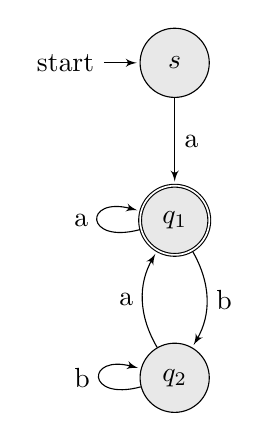
\begin{tikzpicture}[shorten >=1pt,node distance=2cm,auto,>=latex']
    % FSM TiKZ Style
    \tikzstyle{every state}=[fill={rgb:black,1;white,10}]

    % Nodes, positions, and labels
    \node[state,initial]   (s)                  {$s$};
    \node[state,accepting] (q_1) [below of=s]   {$q_1$};
    \node[state]           (q_2) [below of=q_1] {$q_2$};

    % Edges and labels
    \path[->]
    (s)   edge              node {a} (q_1)
    (q_1) edge [loop left]  node {a} (   )
          edge [bend left]  node {b} (q_2)
    (q_2) edge [loop left]  node {b} (   )
          edge [bend left]  node {a} (q_1);

\end{tikzpicture}

\end{document}
